\section{实验与结果}
\label{sec:experiments}

在本节中，我们进行了广泛的实证评估，以验证所提出的多平台混合框架。实验旨在验证四个核心假设：1）约束感知的宏观规划器是否能有效防止液体溢出；2）姿态感知的大规模并行DRL智能体是否能保证直立器材抓取；3）正则化少样本微调管线是否能成功弥合基于IL的微量移液的虚实鸿沟；4）完整系统是否能无缝地端到端自主执行生化化验工作流。

对具有成功次数与试验次数的二元结果，使用Wilson得分法计算95\%置信区间：
\begin{equation}
    \begin{aligned}
    D &= 1+z^2/n,\quad z=1.96,\\
    c &= (\hat p+z^2/(2n))/D,\\
    h &= \frac{z}{D}\sqrt{\frac{\hat p(1-\hat p)}{n}+\frac{z^2}{4n^2}},\\
    \text{CI}_{95\%} &= [c-h,c+h].
    \end{aligned}
\end{equation}
其中$\hat{p}$为观测成功率，$n$为实验次数。
连续指标应在独立样品或回合层面估计不确定性。若无原始配对记录，不能仅凭汇总百分比宣称统计显著。

\subsection{实验平台与硬件配置}
\label{subsec:exp_setup}

物理验证平台严格镜像了Isaac Sim仿真环境。移动操作系统配备了一个差速驱动底盘和一个6自由度UR3机械臂。Robotiq 2F-85平行夹爪安装了定制的柔性橡胶垫，用于固定易碎的玻璃器皿和微孔板。

感知子系统方面，Intel RealSense D435 RGB-D相机以eye-to-hand构型安装，提供连续的点云和视觉反馈。计算管线——包括实时3D体素代价地图生成、DRL策略推理和分层状态机（HSM）序列控制——在本地NVIDIA RTX 4090工作站上执行，通过ROS桥接确保低延迟通信。

\subsection{状态同步实测结果}
\label{subsec:state_sync_eval}
表~\ref{tab:sync_illustrative}列出用户提供的仿真与实体状态接口实测汇总值。按所列汇总值，关节状态一致性、物体位姿误差、更新延迟、观测有效性和抓取状态识别均满足预设目标。物体位姿误差应以独立参考测量计算，不能以更新仿真场景的同一RGB-D估计作为真值。目前尚未获得对应的回合数、原始时间戳轨迹、参考测量方法和不确定性区间，故这些汇总值仍需逐回合记录核验，不能据此进行统计显著性判断。下文任务成功率来自其他实验，不应视为状态同步指标。

\begin{table}[!t]
\caption{状态同步目标与提供的实测汇总结果}
\label{tab:sync_illustrative}
\centering
\resizebox{\columnwidth}{!}{%
\begin{tabular}{lcc}
\hline\hline
\textbf{指标} & \textbf{目标} & \textbf{实测结果} \\ \hline
关节角度平均绝对误差 & $\leq 0.5^\circ$ & $0.42^\circ$ \\
关节角度误差95分位数 & $\leq 1.5^\circ$ & $1.2^\circ$ \\
物体位置误差：静止 & $\leq 3$ mm & $2.2$ mm \\
物体位置误差：运动 & $\leq 5$ mm & $3.4$ mm \\
物体位置误差：短暂遮挡 & $\leq 10$ mm & $8.1$ mm \\
物体姿态误差：运动 & $\leq 4^\circ$ & $3.6^\circ$ \\
更新延迟：中位数/95分位数 & $\leq 50/100$ ms & $41/87$ ms \\
过期或被拒绝观测比例 & $\leq 2\%$ & $1.4\%$ \\
抓取状态识别准确率 & $\geq 98\%$ & $98.7\%$ \\ \hline\hline
\end{tabular}}
\end{table}

\subsection{宏观导航与流体稳定性}
\label{subsec:exp_macro_benchmarks}

为评估宏观安全性，移动底盘被要求在高度杂乱的实验室环境中运输开敞液体容器。我们将本文的约束感知经典规划器与标准RRT*规划器和纯DRL导航策略进行了基准对比。评估指标包括整体成功率、最小障碍间距和平均轨迹冲击（流体晃动的主要指标）。

轨迹平滑度通过平均冲击指标量化：
\begin{equation}
    J_{\text{smooth}} = \frac{1}{T} \sum_{t=1}^{T} \left\| \dddot{\mathbf{q}}_t \right\|^2
\end{equation}
其中$\dddot{\mathbf{q}}_t$是时间步$t$处关节轨迹的三阶导数（冲击）。

\begin{table}[!t]
\renewcommand{\arraystretch}{1.3}
\caption{宏观导航规划器的定量比较}
\label{tab:navigation_metrics}
\centering
\begin{tabular}{lccc}
\hline\hline
\textbf{评估指标} & \textbf{标准RRT*} & \textbf{纯DRL} & \textbf{本文方法} \\ \hline
实验次数 / 成功次数 & 50\,/\,37 & 50\,/\,34 & 50\,/\,\textbf{44} \\
成功率 (\%) & 74.0 & 68.0 & \textbf{88.0} \\
Wilson 95\%区间 (\%) & [60.4,84.1] & [54.2,79.2] & [76.2,94.4] \\
平均轨迹冲击 ($m/s^3$) & 4.52 & 6.18 & \textbf{0.85} \\
最小间距 ($m$) & 0.12 & 0.08 & \textbf{0.28} \\
规划时间 (ms) & 12.3 & \textbf{2.1} & 8.7 \\ \hline\hline
\end{tabular}
\end{table}

表\ref{tab:navigation_metrics}支持本文规划器轨迹加加速度较低的结论，但不能单独证明液体不溢出。真实液体测试应在匹配容器、液体、填充率和路线的条件下，测量运输前后容器与托盘质量（同时控制蒸发和操作损失）、标定侧视相机得到的最大自由液面倾角，以及超过预定溢出阈值的回合比例；需覆盖正常行驶、转弯、急停和遇障重规划。目前这些直接液体测量值尚未提供。

\begin{table}[!t]
\caption{真实液体稳定性结果（待填）}
\label{tab:liquid_stability}
\centering
\begin{tabular}{lccc}
\hline\hline
\textbf{规划器} & \textbf{损失质量(g)} & \textbf{最大液面角} & \textbf{溢出次数/$n$} \\ \hline
RRT* & 待填 & 待填 & 待填 \\
纯DRL & 待填 & 待填 & 待填 \\
约束感知规划 & 待填 & 待填 & 待填 \\ \hline\hline
\end{tabular}
\end{table}

\subsection{面向姿态感知抓取的大规模并行DRL}
\label{subsec:exp_rl_grasping}

抓取未密封的液体药瓶是一项极具挑战的任务，因为在抬升阶段任何显著的倾斜都会导致化验失效。我们评估了在Isaac Sim中训练的大规模并行PPO抓取策略，并进行了消融实验，以单独验证本文提出的"姿态感知乘数（$M_{\text{posture}}$）"的贡献。我们将基线PPO（仅使用标准距离奖励训练）与本文的姿态感知PPO进行了对比。

\begin{table}[!t]
\renewcommand{\arraystretch}{1.3}
\caption{DRL姿态感知奖励机制的消融研究}
\label{tab:rl_grasping}
\centering
\begin{tabular}{lcc}
\hline\hline
\textbf{评估指标} & \textbf{基线PPO} & \textbf{姿态感知PPO} \\ \hline
实验次数 / 成功次数 & 200\,/\,158 & 200\,/\,\textbf{172} \\
抓取成功率 (\%) & 79.0 & \textbf{86.0} \\
Wilson 95\%区间 (\%) & [72.8,84.1] & [80.5,90.1] \\
最大倾斜角 (度) & $35.4^\circ \pm 12.1^\circ$ & $\mathbf{4.2^\circ \pm 1.5^\circ}$ \\
液体溢出率 (\%) & 42.0 & \textbf{0.0} \\
收敛迭代次数 & 8500 & \textbf{5000} \\ \hline\hline
\end{tabular}
\end{table}

表\ref{tab:rl_grasping}的结果凸显了显著的性能提升。基线PPO为了最小化轨迹距离，经常以激进的角度接近药瓶，导致平均抓取倾斜角高达$35.4^\circ$，泼洒率高达42.0\%。通过集成点积姿态乘数，我们的策略成功收敛至严格的垂直"自上而下（top-down）"抓取，将最大倾斜角锐减至仅仅$4.2^\circ$，并在零样本（zero-shot）物理真机部署期间彻底消除了液体泼洒现象。

\subsubsection{姿态权重敏感性分析}
\label{subsec:sensitivity_analysis}

为了研究姿态感知奖励权重的影响，我们通过将姿态乘数系数$\alpha_{\text{posture}}$从0.0变化到1.0来进行敏感性分析。如表\ref{tab:sensitivity}所示，增加$\alpha_{\text{posture}}$显著降低了倾斜角，但由于行为过于保守，可能会略微降低抓取成功率。

\begin{table}[!t]
\renewcommand{\arraystretch}{1.3}
\caption{姿态权重$\alpha_{\text{posture}}$的敏感性分析}
\label{tab:sensitivity}
\centering
\resizebox{\columnwidth}{!}{
\begin{tabular}{lcccc}
\hline\hline
\textbf{$\alpha_{\text{posture}}$} & \textbf{实验/成功} & \textbf{成功率 (\%)} & \textbf{倾斜角 ($^\circ$)} & \textbf{溢出率 (\%)} \\ \hline
0.0 & 200\,/\,162 & 81.0 & $38.5 \pm 14.2$ & 45.0 \\
0.2 & 200\,/\,167 & 83.5 & $18.3 \pm 8.7$ & 12.0 \\
0.5 & 200\,/\,\textbf{172} & \textbf{86.0} & $4.2 \pm 1.5$ & \textbf{0.0} \\
0.8 & 200\,/\,170 & 85.0 & $2.1 \pm 0.8$ & \textbf{0.0} \\
1.0 & 200\,/\,164 & 82.0 & $1.5 \pm 0.6$ & \textbf{0.0} \\ \hline\hline
\end{tabular}
}
\end{table}

最佳平衡在$\alpha_{\text{posture}} = 0.5$时实现，保持高成功率（86.0\%）的同时完全消除了液体溢出。

\subsubsection{并行环境数量的影响}
\label{subsec:parallel_envs}

我们通过改变Isaac Sim中并行环境的数量$N_{\text{env}}$来评估训练效率。表\ref{tab:parallel_envs}显示了收敛速度和最终性能。

\begin{table}[!t]
\renewcommand{\arraystretch}{1.3}
\caption{并行环境数量对训练的影响}
\label{tab:parallel_envs}
\centering
\begin{tabular}{lcccc}
\hline\hline
\textbf{$N_{\text{env}}$} & \textbf{时间 (h)} & \textbf{迭代} & \textbf{实验/成功} & \textbf{成功率 (\%)} \\ \hline
256 & 12.5 & 8000 & 200\,/\,166 & 83.0 \\
1024 & 4.2 & 6500 & 200\,/\,170 & 85.0 \\
4096 & \textbf{1.8} & \textbf{5000} & 200\,/\,\textbf{172} & \textbf{86.0} \\
8192 & 1.5 & 4800 & 200\,/\,171 & 85.5 \\ \hline\hline
\end{tabular}
\end{table}

将$N_{\text{env}}$从256增加到4096可实现$6.9\times$的训练时间加速，同时提高最终性能。进一步增加到8192收益递减，表明超过4096个环境后存在边际递减效应。

\subsection{面向精密微观操作的模仿学习虚实迁移微调}
\label{subsec:exp_il_pipetting}

Panda设备照片已整合于图~\ref{fig:hsm_recovery_mechanism}，此处不再重复展示；设备示意不能替代任务的定量评估。

对于精细微量移液和水滴角滴加等接触密集型任务，我们评估了基于模仿学习（IL）的视觉运动策略。为了分析虚实迁移的有效性，我们在各项独立技能测试中对比了三个变体：1）Vanilla BC（无域随机化的零样本迁移）；2）DR Only（仅在仿真中加入域随机化）；3）本文方法（DR + 少样本微调）（利用$M=10$次真实世界示教进行正则化微调）。

% 按作者要求暂时隐藏原图6。
\iffalse
\begin{figure}[!t]
    \centering
    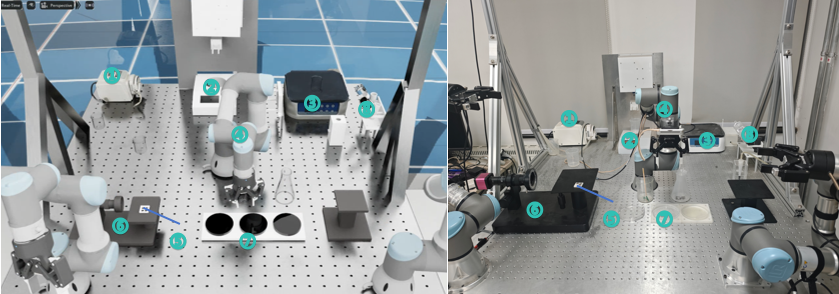
\includegraphics[width=\columnwidth]{images/sim and real.png}
    \caption{实验硬件平台及其在Isaac Sim中的仿真模型，展示了溶液配置、水滴角和梯度稀释工作站。标注组件如下：(1) 水泵——配置溶液时加水；(2) 电子秤——称量所需药品质量；(3) 摇床；(4) UR3机械臂——配置溶液、金属薄膜制备等操作；(5) 金属基材薄膜制备原材料；(6) 水滴角检测装置；(7) 培养皿——放置不同溶液；(8) 所需药品。}
    \label{fig:hardware_setup}
\end{figure}
\fi

\begin{table}[!t]
\renewcommand{\arraystretch}{1.3}
\caption{独立技能测试的虚实迁移IL成功率（非完整工作流）}
\label{tab:il_manipulation}
\centering
\resizebox{\columnwidth}{!}{
\begin{tabular}{lcccccc}
\hline\hline
\textbf{任务} & \multicolumn{2}{c}{\textbf{Vanilla BC}} & \multicolumn{2}{c}{\textbf{DR Only}} & \multicolumn{2}{c}{\textbf{本文方法（完整）}} \\ \hline
 & $n$/成功 & 成功率 & $n$/成功 & 成功率 & $n$/成功 & 成功率 \\
试剂移液 & 50\,/\,20 & 40.0\% & 50\,/\,33 & 66.0\% & 50\,/\,\textbf{42} & \textbf{84.0\%} \\
液滴滴加（水滴角） & 50\,/\,9 & 18.0\% & 50\,/\,29 & 58.0\% & 50\,/\,\textbf{40} & \textbf{80.0\%} \\
梯度稀释对准 & 50\,/\,14 & 28.0\% & 50\,/\,32 & 64.0\% & 50\,/\,\textbf{42} & \textbf{84.0\%} \\ \hline
\textbf{合并技能回合} & 150\,/\,43 & 28.7\% & 150\,/\,94 & 62.7\% & 150\,/\,\textbf{124} & \textbf{82.7\%} \\ \hline\hline
\end{tabular}
}
\end{table}

表\ref{tab:il_manipulation}中三种方法合并技能回合成功率的Wilson 95\%区间依次为[22.0,36.4]\%、[54.7,70.0]\%和[75.8,87.9]\%。本文方法在移液、滴加和稀释各50次测试中的区间分别为[71.5,91.7]\%、[67.0,88.8]\%和[71.5,91.7]\%。这些合并回合不是完整工作流，不能将82.7\%称为端到端成功率。

\subsubsection{补充虚实迁移验证方案}
\label{subsec:transfer_protocol}
为将技能迁移与材料实验可靠性联系起来，补充验证拟选择实际工作流中的精密操作，例如移液或定点滴加，对比仿真BC直接部署、BC加域随机化、以及域随机化加10次完整真实示范正则化微调。固定策略结构、仿真示范集、标称任务设置与测试预算，仅改变域随机化和真实数据微调。各方法采用匹配的初始条件集合，随机安排执行顺序，每次试验后重置工作台，并以多个训练或微调随机种子评估策略间差异。现有汇总表并不能证明这些控制条件和精度测量已经全部实施；本段为待执行的补充方案。

真实示范、验证集与实机测试回合相互独立，测试前冻结策略与验收阈值。初步计划每种方法、每个测试条件至少开展30次独立实机试验，最终样本量依据所需置信区间宽度和对比检验功效确定。报告回合在不同训练策略之间的分配；单个策略的重复试验不能反映训练随机性。

移液使用校准天平测量实际输出质量，按记录温度下的液体密度换算体积，报告有符号偏差、平均绝对相对体积误差及同一目标剂量的输出CV。定点滴加在标定平面上测量实际液滴中心与目标位置的距离；若任务也要求剂量精度，则单独测量剂量误差。预先规定各任务的体积或位置容差，仅当全部精度要求通过且无碰撞、非预期溢出或非计划人工介入时判定成功。保留所有失败回合，完成回合的精度与失败数同时报告，不得静默删除失败样本。报告成功次数/总次数、Wilson 95\%置信区间及精度指标的回合级不确定性。

\subsubsection{少样本效率}
\label{subsec:few_shot}

补充示范数量实验拟固定域随机化预训练策略，对比$M\in\{0,5,10,20\}$次完整真实示范，其中$M=0$为不进行真实微调的DR策略。一次示范指一次完整操作轨迹，而非一帧图像。从仅供训练的示范池构建嵌套子集，并重复子集抽样和不同随机种子的微调；各组使用相同的独立测试条件分布。超参数仅使用验证集选择，测试数据不得参与训练或模型选择。除精度与成功率外，还记录示范采集和微调耗时。该补充方案尚待执行，已有表格中的$M=50$行保留为原有汇总，不代表此次新增实验。

我们分析了真实世界演示数量$M$对微调性能的影响。表\ref{tab:few_shot}展示了不同$M$值的结果。

\begin{table}[!t]
\renewcommand{\arraystretch}{1.3}
\caption{少样本演示数量的影响}
\label{tab:few_shot}
\centering
\begin{tabular}{lccc}
\hline\hline
\textbf{演示数量 ($M$)} & \textbf{实验次数} & \textbf{成功次数} & \textbf{成功率 (\%)} \\ \hline
0 (DR Only) & 50 & 31 & 62.0 \\
5 & 50 & 39 & 78.0 \\
10 & 50 & \textbf{42} & \textbf{84.0} \\
20 & 50 & 42 & 84.0 \\
50 & 50 & 43 & 86.0 \\ \hline\hline
\end{tabular}
\end{table}

现有汇总在$M=10$时给出84.0\%成功率，但不足以确认最优示范数量或具有统计可靠性的性能平台期。作出上述结论前，需要说明具体任务、示范时长、训练随机种子，以及该批次与表\ref{tab:il_manipulation}中测试回合的关系。

\subsubsection{未见条件与泛化测试}
\label{subsec:transfer_generalization}
微调结束后冻结策略，分别测试标称条件、训练随机化范围内的新配置和超出训练范围的条件。优先改变物体初始位置、光照以及硬件兼容的容器尺寸，先开展单因素测试，并明确记录训练和测试的数值范围及真实示范的覆盖情况。只有同时未被仿真随机化和真实微调数据覆盖的条件，才能称为范围外条件；训练范围内的新样本仅证明分布内鲁棒性。实机测试不得超出已验证的硬件安全边界。

各方法和条件使用相同的试验预算与验收规则，报告精度、成功率、相对标称条件的性能变化及失败类别，不能仅以跨条件合并成功率代表泛化。该测试及其数值结果尚待完成，不从已有标称条件成功率推断泛化提升。后续完整薄膜流程保留策略版本与统一运行编号，将操作表现关联到流程成功及薄膜质量，检验精密操作改善是否能转化为合格薄膜产出率的提升。

\subsection{浸涂薄膜制备与材料质量评估}
\label{subsec:exp_dipcoat_quality}

% 按作者要求暂时隐藏原图7及其正文引用。
\iffalse
图~\ref{fig:thin_film_sequence}展示了薄膜处理工作流中机械臂操作干燥烘箱的过程。
\begin{figure*}[!t]
    \centering
    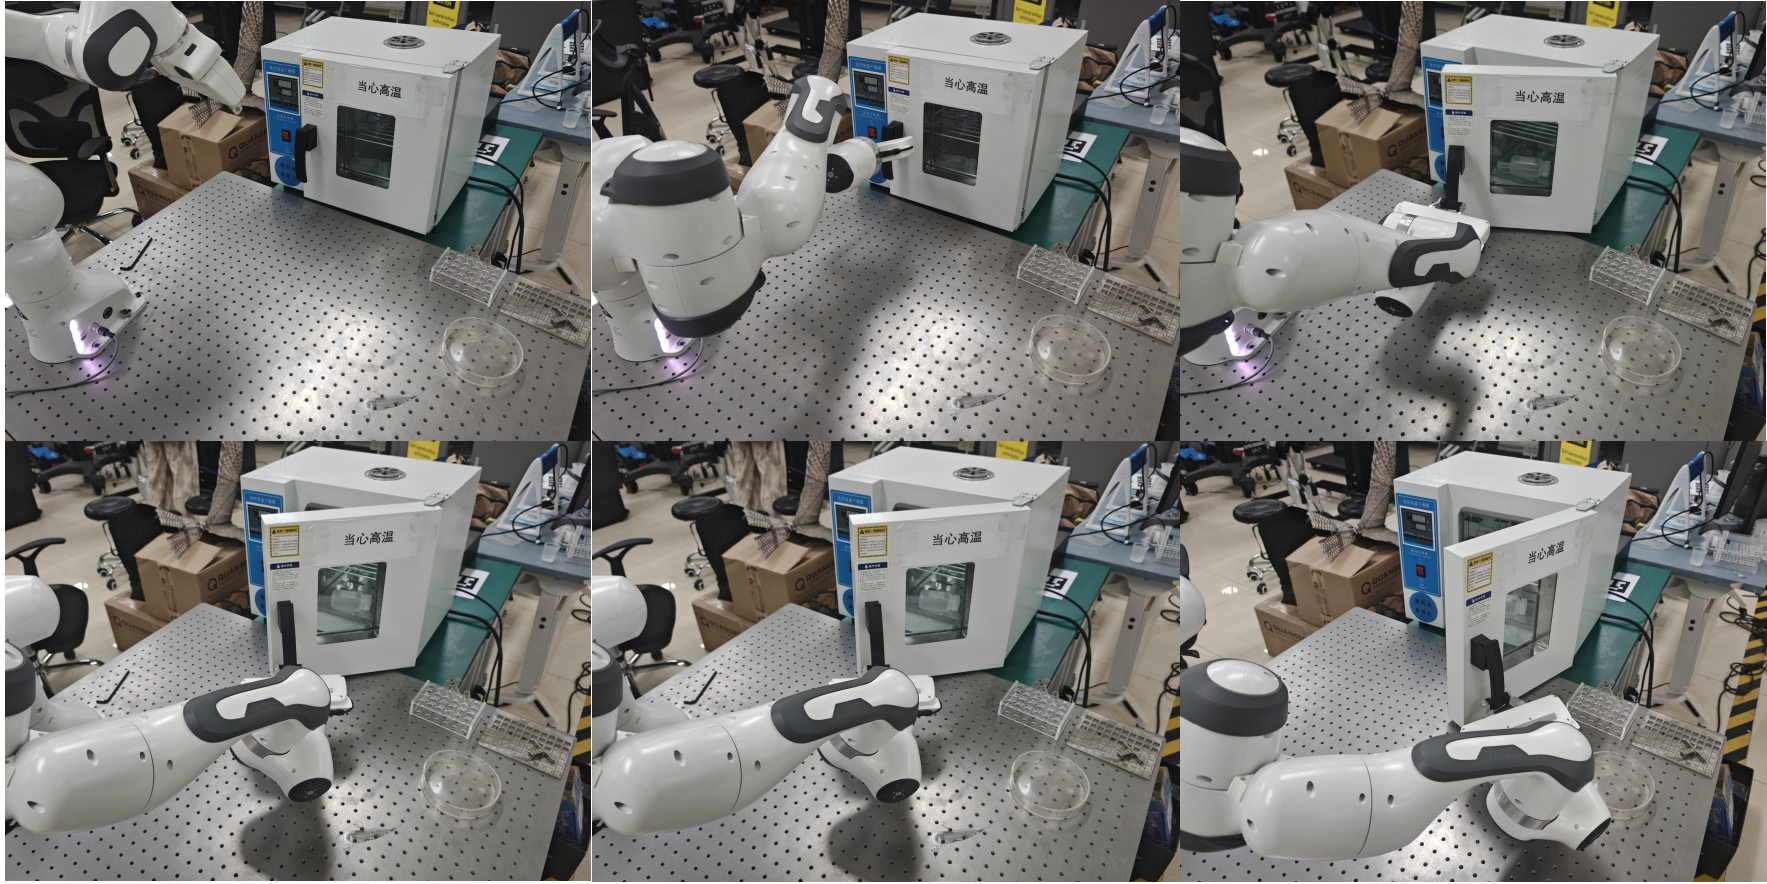
\includegraphics[width=0.9\textwidth]{images/thin_film.png}
    \caption{薄膜处理工作流中的烘箱操作序列，按上排从左到右、再下排从左到右的顺序阅读。图中展示了机械臂接近烘箱、操作门把手及打开烘箱的过程。}
    \label{fig:thin_film_sequence}
\end{figure*}
\fi
已完成的浸涂实验应以材料质量而非仅以机械臂动作成功进行评价。在同一前驱液批次、基底预处理、浸入深度、停留时间、目标提拉速度、干燥/固化条件和测量时间下，比较受训实验人员手工浸涂、机器人固定轨迹与本文学习控制三组。基底应随机分组；条件允许时，材料表征人员应不知道样品所属组别。统计样本量是独立基底数，而非同一基底上的测量点数。

在每片基底的预设位置测量膜厚，以$\mathrm{CV}_{h,i}=100s(h_{ij})/\bar h_i$表示片内膜厚变异系数，并同时报告平均膜厚$\bar h_i$。在规定液滴体积和滴加后等待时间下测量多个位置的静态水接触角，报告均值及空间标准差。采用轮廓仪或AFM，在固定扫描面积内测量表面粗糙度$R_a$或$R_q$。耐腐蚀性测试应统一电解液、暴露面积、温度、稳定时间及电化学流程，报告极化拟合所得腐蚀电流密度$i_{\mathrm{corr}}$；如有EIS数据，再报告低频阻抗$|Z|_{0.01\,\mathrm{Hz}}$。薄膜成功标准应事先按均匀性、附着力与缺陷阈值定义，不能仅凭目视判断。

\begin{table*}[!t]
\renewcommand{\arraystretch}{1.2}
\caption{人工、固定轨迹与学习控制的薄膜质量对比。待取得实测值后填写；不能根据机器人任务成功率推断材料质量。}
\label{tab:film_quality}
\centering
\begin{tabular}{lcccccc}
\hline\hline
\textbf{执行方式} & \textbf{基底数$n$} & \textbf{平均膜厚} & \textbf{膜厚CV (\%)} & \textbf{接触角 ($^\circ$)} & \textbf{粗糙度$R_a$} & \textbf{$i_{\mathrm{corr}}$} \\ \hline
人工操作 & 待填 & 待填 & 待填 & 待填 & 待填 & 待填 \\
机器人固定轨迹 & 待填 & 待填 & 待填 & 待填 & 待填 & 待填 \\
学习控制（本文） & 待填 & 待填 & 待填 & 待填 & 待填 & 待填 \\ \hline\hline
\end{tabular}
\end{table*}

最终表格应补充单位、基底层面的均值$\pm$标准差和95\%置信区间。如有低频阻抗或其他独立防护指标，也应同时报告。三组比较应按数据分布与独立基底设计预先选定统计检验，并对两两比较进行多重检验校正。由于本轮修订尚未获得具体实测值，此处不宣称学习控制在薄膜质量或耐腐蚀性能方面优于基线。

% 跨平台交接实验保留为独立待补内容。

% TODO: 添加跨平台交接实验

% TODO: 添加浸涂质量和交接序列图片
% \begin{figure}[htbp]
%     \centering
%     \includegraphics[width=\columnwidth]{images/dip_coating_results.png}
%     \caption{浸涂薄膜制备的定性结果。}
%     \label{fig:dip_coating_results}
% \end{figure}

% \begin{figure}[htbp]
%     \centering
%     \includegraphics[width=\columnwidth]{images/handover_sequence.png}
%     \caption{基于ArUco定位的跨平台交接序列。}
%     \label{fig:handover_sequence}
% \end{figure}
% ==================== END TODO ====================

% ==================== TODO: P2 - 训练曲线与消融实验（1天） ====================
\subsection{训练收敛与消融研究}
\label{subsec:exp_training_ablation}

% TODO: 添加DRL训练曲线（奖励 vs 迭代次数）
% - 基线PPO vs 姿态感知PPO收敛对比
% - 奖励分解（距离、抓取、抬升、碰撞惩罚）

% \begin{figure}[htbp]
%     \centering
%     % \includegraphics[width=\columnwidth]{images/drl_training_curve.png}
%     \caption{DRL训练收敛曲线。基线PPO与姿态感知PPO的奖励随训练迭代的变化对比。}
%     \label{fig:drl_training_curve}
% \end{figure}

% TODO: 添加IL训练曲线（损失 vs 轮次）
% - 仿真中BC损失收敛
% - 真实示教少样本微调损失

% \begin{figure}[htbp]
%     \centering
%     % \includegraphics[width=\columnwidth]{images/il_training_curve.png}
%     \caption{IL训练损失曲线。仿真中的行为克隆损失与真实世界少样本微调的收敛过程。}
%     \label{fig:il_training_curve}
% \end{figure}

% TODO: 添加消融实验表——各组件贡献
% ==================== END TODO ====================

% ==================== TODO: P2 - SOTA对比（1-2周） ====================
\subsection{与最先进方法的对比}
\label{subsec:exp_sota}

% TODO: 添加SOTA对比表

% TODO: 添加雷达图或多维对比柱状图
% \begin{figure}[htbp]
%     \centering
%     \includegraphics[width=\columnwidth]{images/sota_comparison.png}
%     \caption{与最先进实验室自动化系统的多维度对比。}
%     \label{fig:sota_comparison}
% \end{figure}
% ==================== END TODO ====================

\subsection{端到端自主工作流集成}
\label{subsec:exp_end_to_end}

\subsubsection{失败分类}
每次失败应根据首个未恢复原因赋予唯一主类别：感知、抓取、移液、对接/交接、运输/溢出、通信或恢复次数耗尽。其他促成因素可作为次要标签。按工作流报告各类别失败次数、占全部失败的比例、成功恢复次数及损失时间，避免一次失败重复计数。现有汇总表不足以完成此分析，需逐回合日志。

\subsubsection{科学结果质量与统计检验}
机器人动作完成和实验产物合格应分开报告。溶液制备应报告独立配液的目标/实测浓度误差及移液变异系数（CV）；梯度稀释应报告名义与实测浓度的线性拟合斜率、$R^2$、各级相对误差及阴性对照交叉污染率；薄膜按表\ref{tab:film_quality}报告膜厚CV、接触角偏差、粗糙度与耐腐蚀指标。所有合格阈值须在比较各组结果前确定，并报告同时满足各项阈值的独立运行比例。

关键二元比较应列出成功次数、总次数和Wilson 95\%区间；独立回合可采用双侧Fisher精确检验，配对场景应采用相应的配对精确检验。连续质量指标报告效应量和按独立回合或基底聚类的bootstrap 95\%区间，多组两两比较需作多重检验校正。未获得原始记录前不填写$p$值或伪造聚类置信区间。

为单独检验失败恢复编排的作用，后续应在相同低层技能、初始条件与注入故障下比较：（1）任一状态条件失败即终止的固定顺序状态机；（2）允许有限次数恢复的本文分层状态机。故障应包括抓取失败、对接偏差和过期感知数据。报告试验次数、完整工作流成功率、各阶段失败与恢复率、重试次数、人工干预次数及完成时间。下文现有结果不包含这一消融实验，因此不能用于证明分层状态机优于固定顺序执行。

完整工作流应以同一运行编号从开始追踪到结束，任一阶段失败不得重置分母。分别定义：（1）溶液制备：取试剂、定量配液、混合及质量检测；（2）薄膜制备：溶液送达、基底处理、浸涂、固化及薄膜质量验收；（3）梯度稀释：试剂送达、吸头管理、稀释及浓度/污染检测。仅当全部步骤与科学质量阈值均合格且无计划外人工干预时，才计为完整成功；分别报告首次成功率与恢复后成功率。

下表现有次数是各操作阶段的独立汇总，不能相乘、相加或视为完整流程结果。尤其若均指同一批50次运行，原稿“全循环42/50”与水滴角阶段40/50在逻辑上冲突，须先核对逐回合日志。原稿“连续成功10次”也须有可追溯的运行编号，本次不作为已核实的独立结果。

\begin{table}[!t]
\renewcommand{\arraystretch}{1.3}
\caption{现有阶段级计数；完整工作流结果需逐回合日志核对}
\label{tab:end_to_end}
\centering
\begin{tabular}{lccc}
\hline\hline
\textbf{工作流阶段} & \textbf{实验次数} & \textbf{成功次数} & \textbf{成功率 (\%)} \\ \hline
自主转移 & 50 & 44 & 88.0 \\
直立抓取 & 50 & 43 & 86.0 \\
试剂移液 & 50 & 42 & 84.0 \\
水滴角测量 & 50 & 40 & 80.0 \\
梯度稀释 & 50 & 42 & 84.0 \\ \hline
\textbf{完整工作流} & \textbf{待核对} & \textbf{待核对} & \textbf{待核对} \\ \hline\hline
\end{tabular}
\end{table}

\begin{table}[!t]
\caption{完整工作流结果填写模板（独立运行）}
\label{tab:workflow_complete}
\centering
\begin{tabular}{lccc}
\hline\hline
\textbf{流程} & \textbf{运行数} & \textbf{首次成功} & \textbf{恢复后成功} \\ \hline
溶液制备 & 待填 & 待填 & 待填 \\
薄膜制备 & 待填 & 待填 & 待填 \\
梯度稀释 & 待填 & 待填 & 待填 \\ \hline\hline
\end{tabular}
\end{table}

% \begin{figure*}[!t]
%     \centering
%     % \includegraphics[width=\textwidth]{figures/end_to_end_snapshots.png}
%     \caption{自主三阶段实验室工作流的顺序快照：(a)--(b) 直立器材抓取和试剂移液；(c)--(d) 约束感知转移和用于水滴角检测的液滴滴加；(e)--(f) 高精度梯度稀释和微孔板对准。}
%     \label{fig:sequential_snapshots}
% \end{figure*}
